\documentclass[11pt,letterpaper]{article}
\usepackage[margin=0.9in]{geometry}
\usepackage[T1]{fontenc}
\usepackage[utf8]{inputenc}
\usepackage{lmodern,microtype,amsmath,amssymb,amsthm,bm}
\usepackage{graphicx,booktabs,enumitem,caption}
\usepackage[authoryear,round]{natbib}
\usepackage[hidelinks]{hyperref}
% Shared expressions keep the manuscript and poster conventions identical.
\newcommand{\ejab}{\mathit{eJAB}}
\newcommand{\BF}{\mathit{BF}}
\newcommand{\TSBF}{\mathit{TSBF}}
\newcommand{\BFF}{\mathit{BFF}}
\newcommand{\Hnull}{\mathcal H_0}
\newcommand{\Halt}{\mathcal H_1}
\newcommand{\Hplus}{\mathcal H_+}
\newcommand{\Normal}{\mathcal N}
\newcommand{\pto}{\xrightarrow{P}}
\newcommand{\dto}{\xrightarrow{D}}
\newcommand{\TwoSidedFormula}{\sqrt n\exp\!\left\{-\frac12
  \left(1-n^{-1/q}\right)Q_{\chi_q^2}(1-p)\right\}}
\newcommand{\OneSidedFormula}{\frac{\sqrt n\exp\!\left\{
  -\frac12 Q_{\chi_1^2}(1-p)\right\}}{2(1-p_1)}}
\newcommand{\ReconstructedP}{p=2\min\{p_1,1-p_1\}}
\newcommand{\NullPrior}{\theta\mid\Halt\sim\Normal(\theta_0,nv_n)}
\newcommand{\GaussianPosterior}{\theta\mid\boldsymbol y,\Halt
  \ \dot\sim\ \Normal(\widehat\theta,v_n)}
\newcommand{\Rone}{\Pr(p_n\leq\delta\mid\Hnull)\longrightarrow C\delta,
  \quad 0<\delta\leq U_p}
\newcommand{\Rtwo}{D_{q,n}=\sqrt n\,
  \begin{cases}
   -p_n\log p_n,&q=1,\\
   p_n,&q\geq2
  \end{cases}
  \pto0}
\newcommand{\EWDE}{\operatorname{EWDE}}
\newcommand{\NormalizedEWDE}{\operatorname{EWDE}_{\mathrm{norm}}}

\graphicspath{{figures/}}
\setlength{\parindent}{0pt}
\setlength{\parskip}{5pt}
\setlength{\emergencystretch}{2em}
\setlength{\bibsep}{4pt}
\captionsetup{font=small,labelfont=bf}
\newtheorem{theorem}{Theorem}
\newcommand{\drafttitle}{Further developments of generalized Jeffreys's approximate Bayes factor}
\hypersetup{pdftitle={\drafttitle: one-sided eJAB, regularity and Equally Weighted Decision Error Profiles},
  pdfauthor={Zhengxiao Wei and coauthors}}

\begin{document}
\begin{center}
{\LARGE\bfseries Further developments of generalized\\
Jeffreys's approximate Bayes factor\par}
\vspace{5pt}
{\large One-sided eJAB, regularity and Equally Weighted Decision Error Profiles\par}
\vspace{12pt}
Zhengxiao Wei$^1$, Puneet Velidi$^1$, Evan Strasdin$^1$,\\
Shreena Nisha Kalaria$^2$, Yimeng Liu$^1$, C\'eline M.~Laumont$^2$,\\
Brad H.~Nelson$^2$ and Farouk S.~Nathoo$^1$
\vspace{6pt}

{\small $^1$Department of Mathematics and Statistics, University of Victoria\\
$^2$Deeley Research Centre, British Columbia Cancer Agency}
\vspace{8pt}

{\small Methods draft for poster development \qquad 16 October 2026}
\end{center}

\begin{abstract}
We further develop and exposit generalized Jeffreys's approximate Bayes
factor (eJAB; Velidi and Wei, 2025). Equally Weighted Decision Error
Profiles compare eJAB with test-statistic Bayes factors (TSBF; Johnson,
2005; Johnson et al., 2023), BIC, and NHST significance rules.
For \(2\times2\) and \(3\times3\) Pearson chi-squared independence tests,
eJAB generally outperforms estimated-\(\omega\) TSBF outside small-sample
or weak-signal regimes; the trend reverses for \(5\times5\) tables.
With true \(\omega\), eJAB generally matches or underperforms TSBF.
BIC differences are small for single-parameter tests; eJAB gains at
weaker effects in multiparameter tests, whereas BIC benefits at stronger
effects. Against \(p<.05\), eJAB gains with larger samples and stronger
signals; weak signals and some small-sample settings favor NHST.
We derive a null-centered one-sided eJAB via the Marsman--Wagenmakers
correction and weaken regularity conditions while retaining consistency.
Three clinical examples illustrate significant findings favoring the null.

\end{abstract}
\nocite{velidi2025generalized}

\section{The unrestricted eJAB definition}
For testing \(\Hnull:\boldsymbol\theta=\boldsymbol\theta_0\) against
\(\Halt:\boldsymbol\theta\ne\boldsymbol\theta_0\), define
\begin{equation}
  \ejab_{01}=\TwoSidedFormula,
  \qquad \ejab_{10}=\ejab_{01}^{-1}.
  \label{eq:two-sided}
\end{equation}
Here \(q\) is the dimension of the test, \(n\) is the sample-size quantity
appropriate to that test, \(p\) is its \(p\)-value, and \(Q_{\chi_q^2}\) is
the chi-squared quantile function. Values greater than one favor the null.
The factor \(1-n^{-1/q}\) is retained in this unrestricted definition.

For unrestricted eJAB, the generalized unit-information prior is
\begin{equation}
 \boldsymbol\theta\mid\Halt\sim
 \Normal_q\!\left(\widehat{\boldsymbol\theta},
 n^{1/q}\mathbf J_n^{-1}(\widehat{\boldsymbol\theta})\right),
 \label{eq:general-prior}
\end{equation}
where \(\widehat{\boldsymbol\theta}\) is the maximum likelihood estimate and
\(\mathbf J_n\) is the observed information in the full sample.
With an asymptotic Gaussian posterior and compatible nuisance-parameter
priors, the Savage--Dickey density ratio gives the approximate Bayes-factor
interpretation \citep{mulder2022generalization}. Setting the covariance
multiplier to \(n^{1/q}\) gives the \(\sqrt n\) prefactor independently of
\(q\).

\section{One-sided construction under a null-centered prior}
\subsection{Prior specification and Gaussian approximation}
For a scalar directional test, consider
\begin{equation}
 \Hnull:\theta=\theta_0
 \qquad\text{versus}\qquad
 \Hplus:\theta>\theta_0 .
 \label{eq:hypotheses}
\end{equation}
Start with an encompassing unrestricted alternative \(\Halt\), and let
\(v_n=I_n^{-1}(\widehat\theta)\) denote the inverse observed information in
the full sample. The construction used here takes the prior to be
centered at the null:
\begin{equation}
 \NullPrior,
 \qquad
 \GaussianPosterior.
 \label{eq:null-centered}
\end{equation}
The second expression is the leading Gaussian posterior approximation.
The prior location is \(\theta_0\); the approximate posterior location is
\(\widehat\theta\).

Under the Savage--Dickey representation, with the required compatibility
of nuisance-parameter priors, the scalar Gaussian density ratio becomes
\begin{align}
 \widetilde{\BF}_{01}^{(0)}
 &=
 \frac{\phi(\theta_0;\widehat\theta,v_n)}
      {\phi(\theta_0;\theta_0,nv_n)}
 =\sqrt n\exp\!\left\{-\frac12 W\right\},
 \label{eq:null-ratio}\\
 W&=\frac{(\widehat\theta-\theta_0)^2}{v_n}.
 \nonumber
\end{align}
Here \(\phi(\,\cdot\,;\mu,v)\) denotes a normal density with mean \(\mu\)
and variance \(v\). The tilde identifies the Gaussian approximation,
and the superscript identifies the null-centered construction. This is
the unrestricted base used to obtain the directional approximation below.

\subsection{Restriction to the predicted direction}
The symmetric encompassing prior assigns probability \(1/2\) to
\(\theta>\theta_0\). For a moderate sample size and a relatively vague
prior, the one-sided \(p\)-value \(p_1\) gives the approximate posterior
mass in that direction \citep{marsman2017three,wagenmakers2022approximate}:
\begin{equation}
 \Pr(\theta>\theta_0\mid\Halt)=\frac12,
 \qquad
 \Pr(\theta>\theta_0\mid\boldsymbol y,\Halt)\approx1-p_1.
 \label{eq:mass}
\end{equation}
The encompassing-prior identity and Bayes-factor composition give
\begin{equation}
 \BF_{+1}
 =\frac{\Pr(\theta>\theta_0\mid\boldsymbol y,\Halt)}
        {\Pr(\theta>\theta_0\mid\Halt)}
 \approx2(1-p_1),
 \qquad
 \BF_{0+}=\frac{\BF_{01}}{\BF_{+1}}.
 \label{eq:restriction}
\end{equation}
Reconstruct the two-sided value as \(\ReconstructedP\) and substitute
\(Q_{\chi_1^2}(1-p)\) for \(W\). The resulting one-sided eJAB is
\begin{equation}
 \boxed{\ejab_{0+}=\OneSidedFormula.}
 \label{eq:one-sided}
\end{equation}
The directional factor retains the information about which side of the
null is supported by the data. Equation~\eqref{eq:one-sided} compares the
point null in Equation~\eqref{eq:hypotheses} with the directional
alternative.

\subsection{Finite-sample convention}
Equation~\eqref{eq:one-sided} omits the factor \((n-1)/n\) from the
exponent and retains \(1/\{2(1-p_1)\}\). This convention follows the
null-centered Gaussian/Savage--Dickey calculation in
Equation~\eqref{eq:null-ratio}; it is an approximation, not an exact
finite-sample conjugate Bayes factor.

The unrestricted definition in Equation~\eqref{eq:two-sided} continues
to use \(1-n^{-1/q}\), which is \((n-1)/n\) when \(q=1\).
Its MLE-centered prior in Equation~\eqref{eq:general-prior} is distinct
from the null-centered prior in Equation~\eqref{eq:null-centered}.
Thus, the displayed one-sided formula is not obtained by dividing the
finite-sample-corrected Equation~\eqref{eq:two-sided} by \(2(1-p_1)\).

\section{Regularity conditions and model-selection consistency}
The approximate Bayes-factor derivation uses an asymptotically Gaussian
posterior and the stated prior. The consistency statement for
Equation~\eqref{eq:two-sided} concerns the behavior of the \(p\)-values.
For fixed integer \(q\geq1\), the revised conditions are
\begin{align}
 \textbf{R1$'$:}\quad &\Rone, \label{eq:r1}\\
 \textbf{R2:}\quad &p_n\pto0,\qquad \Rtwo
 \quad\text{under a fixed }\Halt .
 \label{eq:r2}
\end{align}
In R1$'$, \(U_p\in(0,1]\) and \(0<C\leq1/U_p\) are constants, and
the limit holds for every fixed \(\delta\in(0,U_p]\). Only left-tail
calibration is required; full asymptotic uniformity is the special case
\(U_p=C=1\). R2 retains the original rate when \(q=1\), but removes
the logarithmic factor for integer \(q>1\). It remains stronger than
\(p_n\pto0\) alone. These updates are recorded in the reviewer-response
revision work plan.

\begin{theorem}[Consistency of unrestricted eJAB]
For fixed integer \(q\geq1\), under R1$'$ and the revised R2,
\begin{equation}
 \ejab_{01}\pto
 \begin{cases}
  \infty,&\text{under }\Hnull,\\
  0,&\text{under the fixed alternative }\Halt .
 \end{cases}
 \label{eq:consistency}
\end{equation}
\end{theorem}

\begin{proof}[Proof sketch]
Write \(W_n=Q_{\chi_q^2}(1-p_n)\) and \(a_n=1-n^{-1/q}\).
Under R1$'$, for any fixed \(\delta\in(0,U_p]\),
\[
 \Pr\!\left(W_n>Q_{\chi_q^2}(1-\delta)\mid\Hnull\right)
 \leq\Pr(p_n\leq\delta\mid\Hnull)\longrightarrow C\delta.
\]
Taking \(\delta\) sufficiently small gives \(W_n=O_P(1)\). Hence
\begin{equation}
 \log\ejab_{01}=\tfrac12\log n-\tfrac12 a_n W_n
 \pto\infty .
 \label{eq:null-proof}
\end{equation}

For \(q=1\), the original small-\(p\) chi-squared quantile bound is
\begin{equation}
 Q_{\chi_1^2}(1-p)>
 -2\log p-2\log(-\log p).
 \label{eq:tail-bound}
\end{equation}
For \(q\geq2\), stochastic ordering of chi-squared distributions gives
the sharper bound
\begin{equation}
 Q_{\chi_q^2}(1-p)\geq Q_{\chi_2^2}(1-p)=-2\log p.
 \label{eq:tail-bound-multidimensional}
\end{equation}
This follows by writing a \(\chi_q^2\) variable as a \(\chi_2^2\)
variable plus an independent nonnegative \(\chi_{q-2}^2\) variable
when \(q>2\); equality holds when \(q=2\).
Define \(b_q(p)=-p\log p\) for \(q=1\) and \(b_q(p)=p\) for
\(q\geq2\), so \(D_{q,n}=\sqrt n\,b_q(p_n)\).
Because \(p_n\pto0\), the relevant bound applies with probability
tending to one. Both cases yield
\begin{align}
 0<\ejab_{01}
 &\leq \sqrt n\,[b_q(p_n)]^{a_n}\nonumber\\
 &=n^{1/(2n^{1/q})}D_{q,n}^{\,1-n^{-1/q}}\pto0 .
 \label{eq:alternative-proof}
\end{align}
The last step uses \(n^{1/(2n^{1/q})}\to1\), \(D_{q,n}\pto0\), and an
exponent tending to one.
\end{proof}

\subsection{Fixed and local alternatives}
A prior centered at the null and a sequence of local alternatives are
different specifications. Consider sequences of the form
\(\theta_n=\theta_0+c/\sqrt n\). For regular tests, these may
produce a nondegenerate noncentral chi-squared limit, so \(p_n\) need not
converge to zero and R2 need not hold. The consistency statement above
therefore does not give consistency along all such local sequences.

Johnson's original local-alternative TSBF differs from the later
nonlocal-prior Bayes factor function
\citep{johnson2005bayes,johnson2023bff}. For every fixed nonzero
effect-size ordinate, the latter has pointwise model-selection
consistency. These distinctions determine which asymptotic claims apply
to a given comparison.

\section{Equally Weighted Decision Error Profiles}
\subsection{Definition and decision rules}
For each effect size \(\theta\) and sample size \(n\), compare a simple
null with effect zero and a simple alternative with effect \(\theta\).
Under \(0\)--\(1\) loss, the equally weighted decision error (EWDE) of
decision rule \(d\) is
\begin{equation}
 \EWDE_d(\theta,n)=
 \frac{\alpha_d(\theta,n)+\beta_d(\theta,n)}{2},
 \label{eq:ewde}
\end{equation}
where \(\alpha_d\) is the type I error probability under the null and
\(\beta_d\) is the type II error probability at the specified
alternative. The profiles display the normalized EWDE comparison,
defined by
\begin{align}
 \Delta E(\theta,n)&=\EWDE_{\mathrm{comparison}}(\theta,n)
                         -\EWDE_{\ejab}(\theta,n),\nonumber\\
 \NormalizedEWDE(\theta,n)&=\frac{\Delta E(\theta,n)}{M},
 \qquad
 M=\max_{(\theta,n)\in\mathcal G}|\Delta E(\theta,n)| .
 \label{eq:normalized-ewde}
\end{align}
The grid \(\mathcal G\) and normalization constant \(M\) are specific to
each panel. Positive values favor eJAB and negative values favor the
comparison rule. The shared color scale is \([-1,1]\), and the printed
\(M\) values retain the scale of the underlying EWDE differences.
The calculation is pointwise in effect size, rather than integrated over
a composite alternative prior.

The profiles use the unrestricted rule \(\ejab_{01}\leq1\).
Figure~\ref{fig:main-ewde} compares it with the TSBF rules and \(p<.05\).
The Bayes-factor threshold of one corresponds to equal prior model
probabilities and \(0\)--\(1\) loss. Figure~\ref{fig:additional-ewde}
compares eJAB with \(p<.005\) and the BIC Bayes-factor rule.

\subsection{Test-statistic Bayes-factor comparisons}
The chi-squared comparison uses the Bayes factor function of
\citet{johnson2023bff}, given by
\begin{align}
 \BFF_{10}(x_n\mid\tau^2)
 &=(1+\tau^2)^{-q/2-1}
   \left(1+\frac{\tau^2x_n}{q(1+\tau^2)}\right)
   \exp\!\left\{\frac{\tau^2x_n}{2(1+\tau^2)}\right\},
 \label{eq:bff}\\
 \tau_\omega^2&=\frac{n\omega^2}{q}.
 \nonumber
\end{align}
Here \(\omega\) is the standardized effect-size ordinate. The main figure
includes the prespecified-effect rule and its estimated-effect
sensitivity version for \(2\times2\), \(3\times3\) and \(5\times5\)
contingency tables.

Panel A estimates the effect by \(\widehat\omega=\sqrt{X^2/n}\), so
\(\widehat\tau^{\,2}=X^2/q\). Since
\(X^2=Q_{\chi_q^2}(1-p)\), this plug-in estimate is recoverable from
the same observed \(p,n,q\) inputs as eJAB. Panel B instead evaluates
the rule at the true effect for each comparison setting.

For any fixed \(\omega>0\), the displayed Bayes factor is increasing
in \(X^2\). The monotone likelihood ratio of the noncentral chi-squared
family therefore makes its upper-tail rejection rule uniformly most
powerful among \(X^2\)-based tests at its attained size. This
Neyman--Pearson argument \citep{fowlie2021neyman} concerns power at a
specified size. Separately, cutoff one minimizes prior-predictive error
under fixed model priors, equal model probabilities and \(0\)--\(1\)
loss; it does not guarantee optimal pointwise average error at each true
effect size. The plug-in Panel A remains a sensitivity analysis.

For Pearson chi-squared tests of independence in \(2\times2\) and
\(3\times3\) tables, eJAB generally has lower EWDE than the
estimated-\(\omega\) TSBF outside small-sample or weak-signal regimes.
In \(3\times3\) tables, small samples can favor TSBF even at larger
effects. The broad pattern reverses for \(5\times5\) tables: estimated-effect
TSBF generally has lower EWDE, with eJAB gains concentrated in a band of
weaker effects. When TSBF uses the true \(\omega\), eJAB is generally
comparable or worse. The differences are not uniformly small near weak
signals, and the few regions favoring eJAB do not establish dominance.

\subsection{BIC and NHST comparisons}
For BIC, the single-parameter comparisons (\(t\)-tests, linear regression
and logistic regression) show small absolute EWDE differences. In ANOVA,
repeated-measures ANOVA and chi-squared independence tests, eJAB's largest
gains occur in weaker-effect bands that move toward zero as sample size
increases. At stronger effects, where both rules have high power, BIC's
lower Type I error can yield lower EWDE; these differences tend to diminish
at larger samples.

Against the NHST significance rule \(p<.05\), eJAB generally gains with
larger samples and sufficiently strong signals. NHST can have lower EWDE
in weak-signal bands. Small-sample behavior also depends on dimension:
for multiparameter tests, eJAB can gain at intermediate effects while
NHST gains at stronger effects. The normalized profiles show relative
patterns; each panel's \(M\) records the absolute EWDE scale.

\subsection{Local-alternative contours}
Dashed curves follow \(\theta=c/\sqrt n\), with \(\theta=\omega\)
for table comparisons. They hold \(\sqrt n\,\theta\) fixed and hence
preserve alternative test-statistic distributions that depend on
\(n,\theta\) through this quantity. The eJAB threshold also depends on
\(n\), so the curves need not have constant normalized EWDE.

\section{Clinical-trial illustration}
The revised retrospective analysis uses the August 7, 2025
ClinicalTrials.gov snapshot and retains 16,563 primary- and
secondary-outcome analyses from 1,790 exact Early Phase I, Phase I and
Phase II interventional trials. Combined-phase trials and Phase III
and IV trials are excluded. The 427 explicitly one-sided scalar
analyses use Equation~\eqref{eq:one-sided}; the remaining 16,136 use
the unrestricted definition with its finite-sample correction.

Table~\ref{tab:clinical-contradictions} transfers the three illustrative
cases from the revised manuscript. Each finding is statistically
significant while the applicable eJAB favors the null. These examples
span Early Phase I, Phase I and Phase II trials.

\begin{table}[htbp]
\centering
\setlength{\tabcolsep}{4pt}
\begin{tabular}{@{}p{1.18in}p{2.35in}rrr@{}}
\toprule
Trial and phase & Outcome and comparison & \(n\) & \(p\) & \(\ejab\)\\
\midrule
\href{https://clinicaltrials.gov/study/NCT00494806?tab=results}{NCT00494806}\newline Early Phase I & First flatus: rocking vs standard care; \(t\)-test & 66 & \(<.05\) & 1.23\\[6pt]
\href{https://clinicaltrials.gov/study/NCT03907683?tab=results}{NCT03907683}\newline Phase I & Activity after a weekday move-more message; \(t\)-test & 80 & .037 & 1.04\\[6pt]
\href{https://clinicaltrials.gov/study/NCT00539539?tab=results}{NCT00539539}\newline Phase II & CPR fraction: feedback on vs off; linear regression & 1,586 & .016 & 2.19\\
\bottomrule
\end{tabular}
\caption{Three illustrative clinical-trial contradictions transferred
from the revised manuscript. CPR denotes cardiopulmonary resuscitation.
For the first case, the eJAB calculation uses the reported bound \(.05\).}
\label{tab:clinical-contradictions}
\end{table}

This exploratory reanalysis uses reported numerical bounds, such as
\(.05\) for \(p<.05\), to compute eJAB while retaining inequalities
for significance. Bounds can overstate null evidence, so classifications
are provisional. Contradictions establish neither a true null nor a
Type I error.

\clearpage
\begin{figure}[p]
\centering
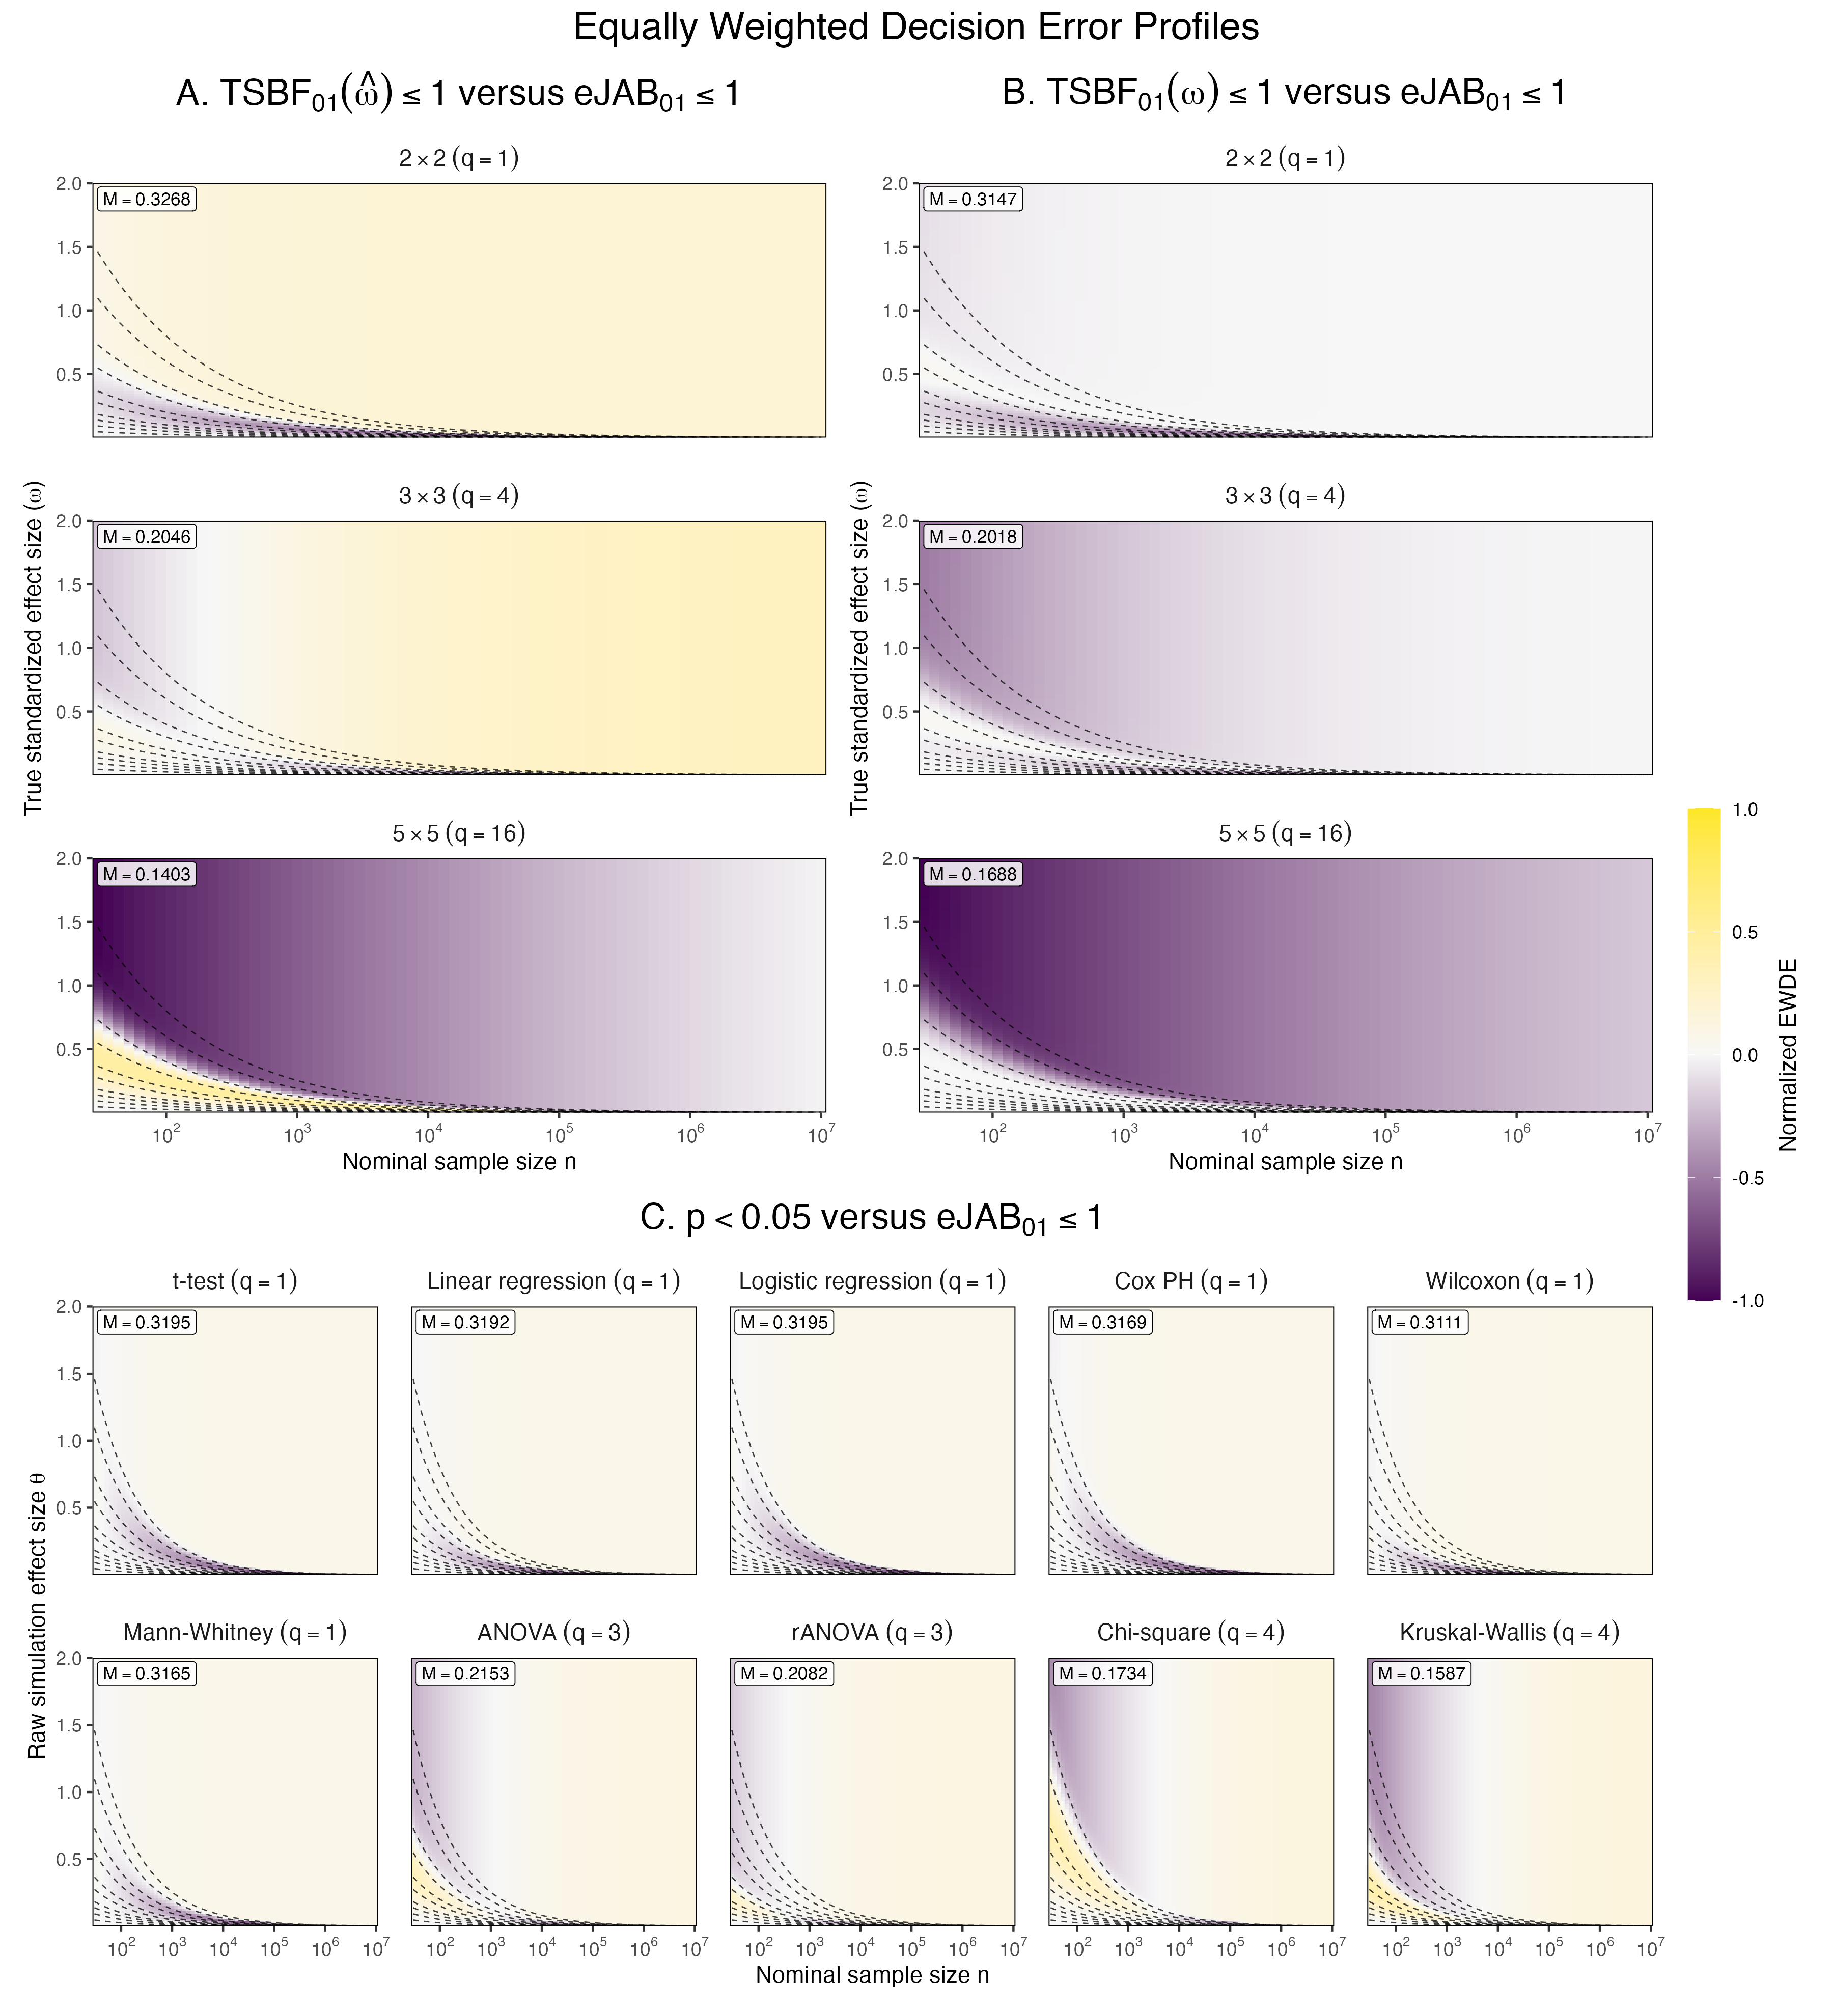
\includegraphics[width=\textwidth]{ewde_main.png}
\caption{Equally Weighted Decision Error Profiles.
(A) \(\TSBF_{01}(\widehat\omega)\leq1\) and
(B) \(\TSBF_{01}(\omega)\leq1\), each versus \(\ejab_{01}\leq1\), for
\(2\times2\), \(3\times3\) and \(5\times5\) contingency tables.
(C) \(p<.05\) versus \(\ejab_{01}\leq1\) across ten statistical tests.
Colors show normalized EWDE: yellow favors eJAB; purple favors the comparison rule.
Each panel reports its normalization constant \(M\). Dashed curves show
\(\theta=c/\sqrt n\), with \(\theta=\omega\) in (A) and (B).
The figure uses unrestricted eJAB.}
\label{fig:main-ewde}
\end{figure}
\clearpage
\begin{figure}[p]
\centering
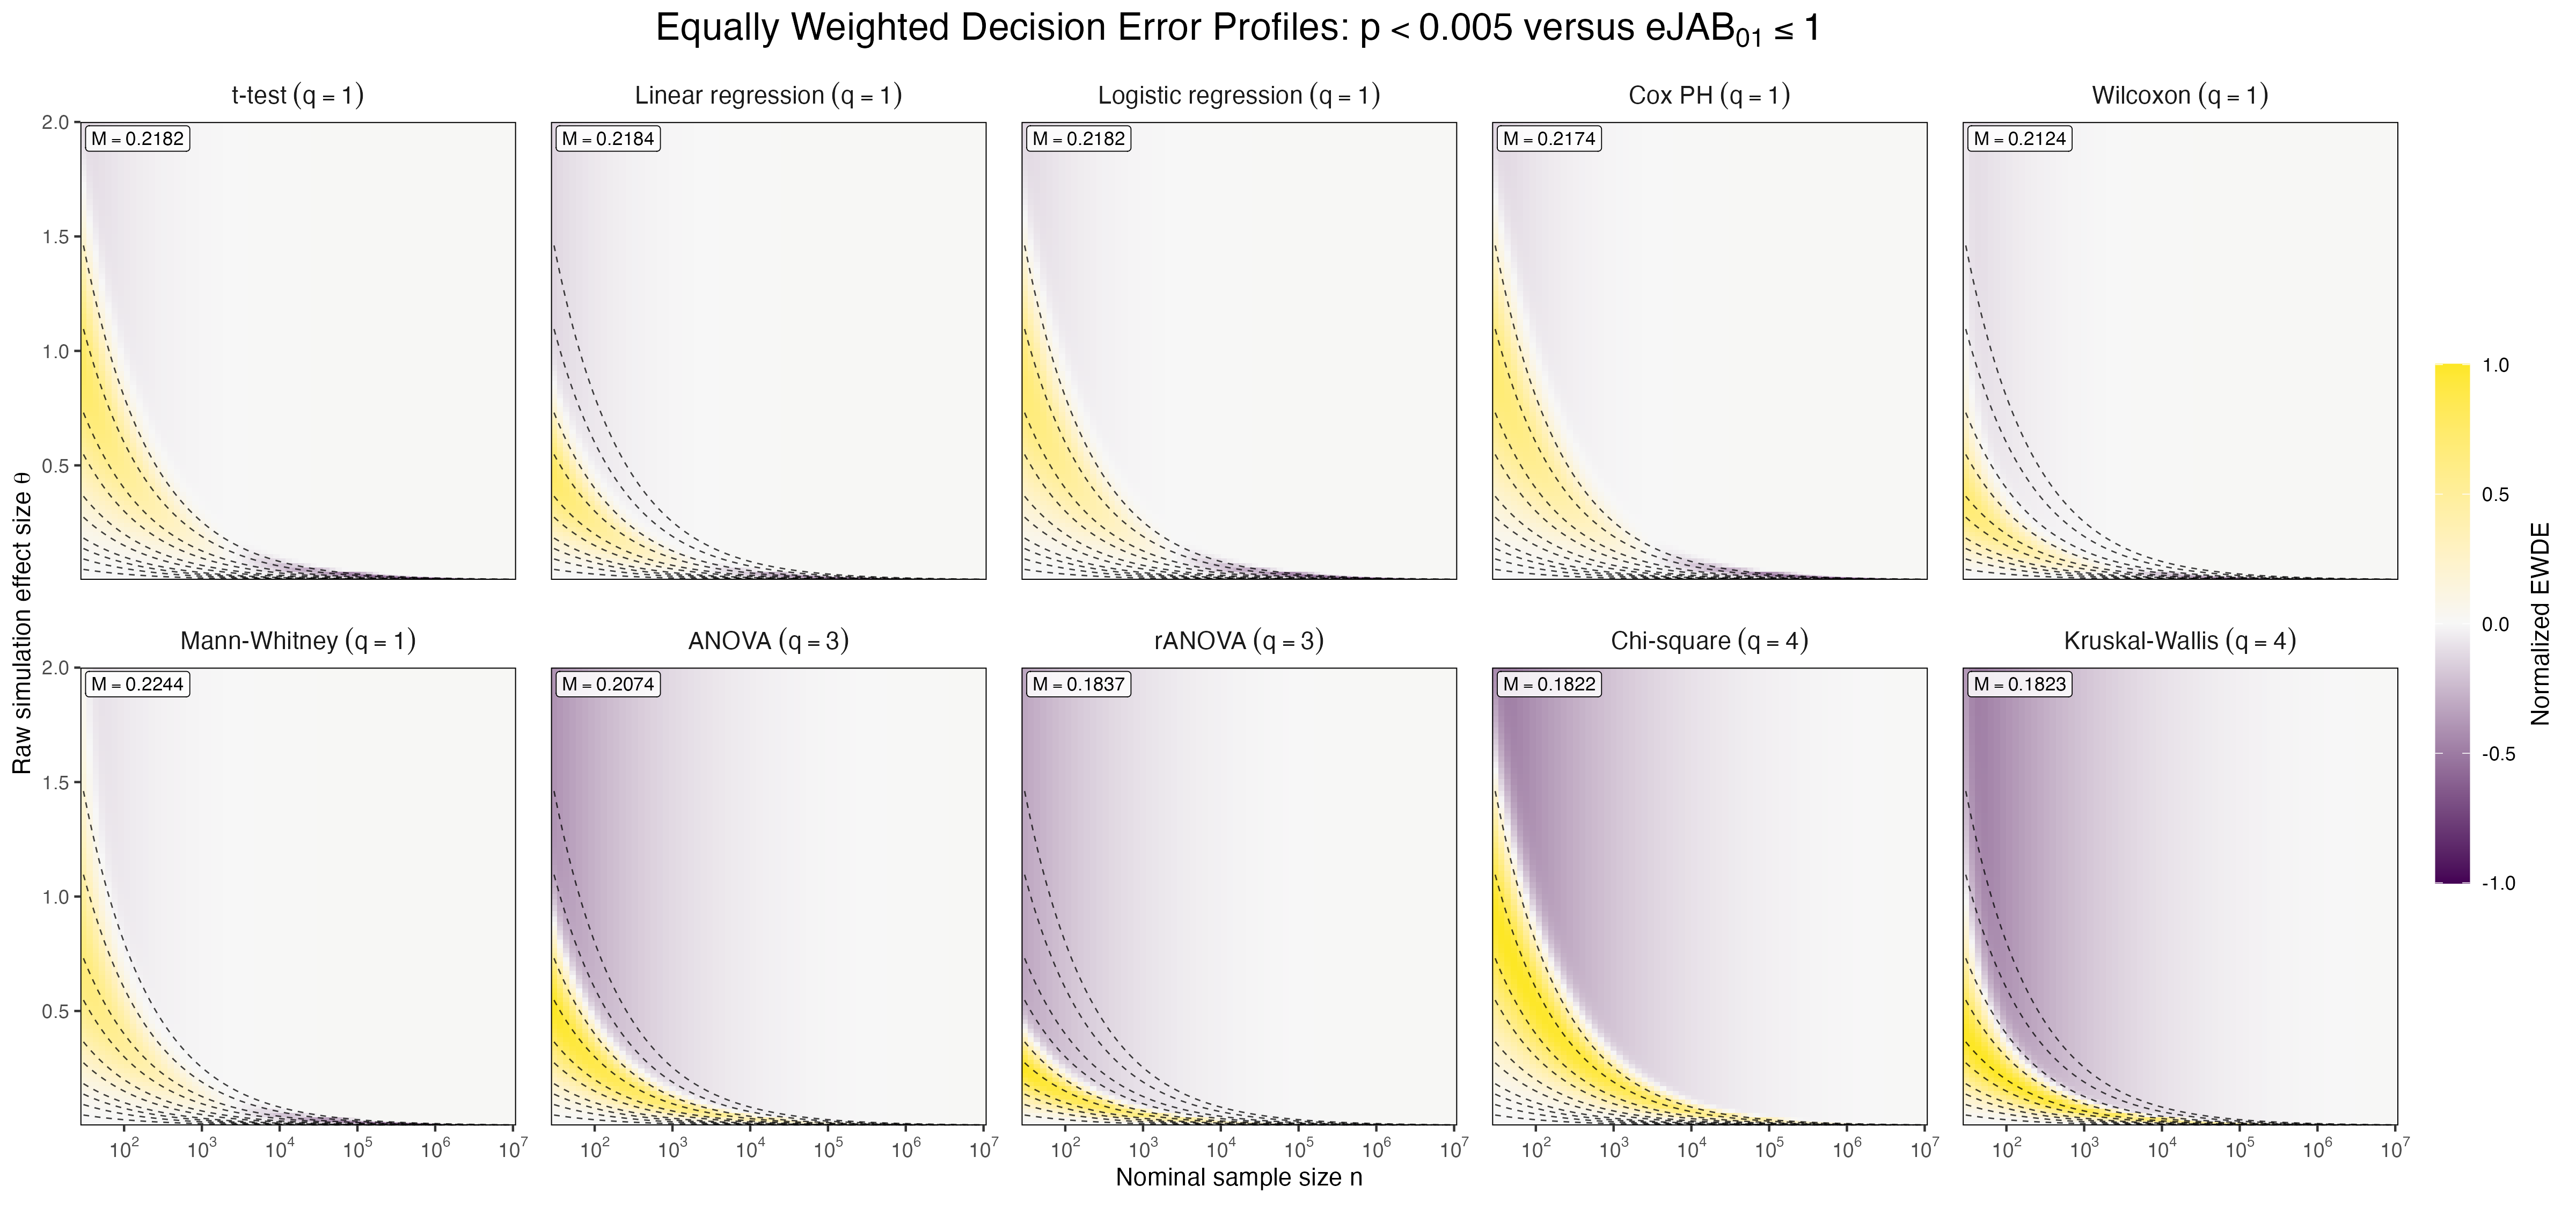
\includegraphics[width=\textwidth]{ewde_p005.png}
\vspace{8pt}

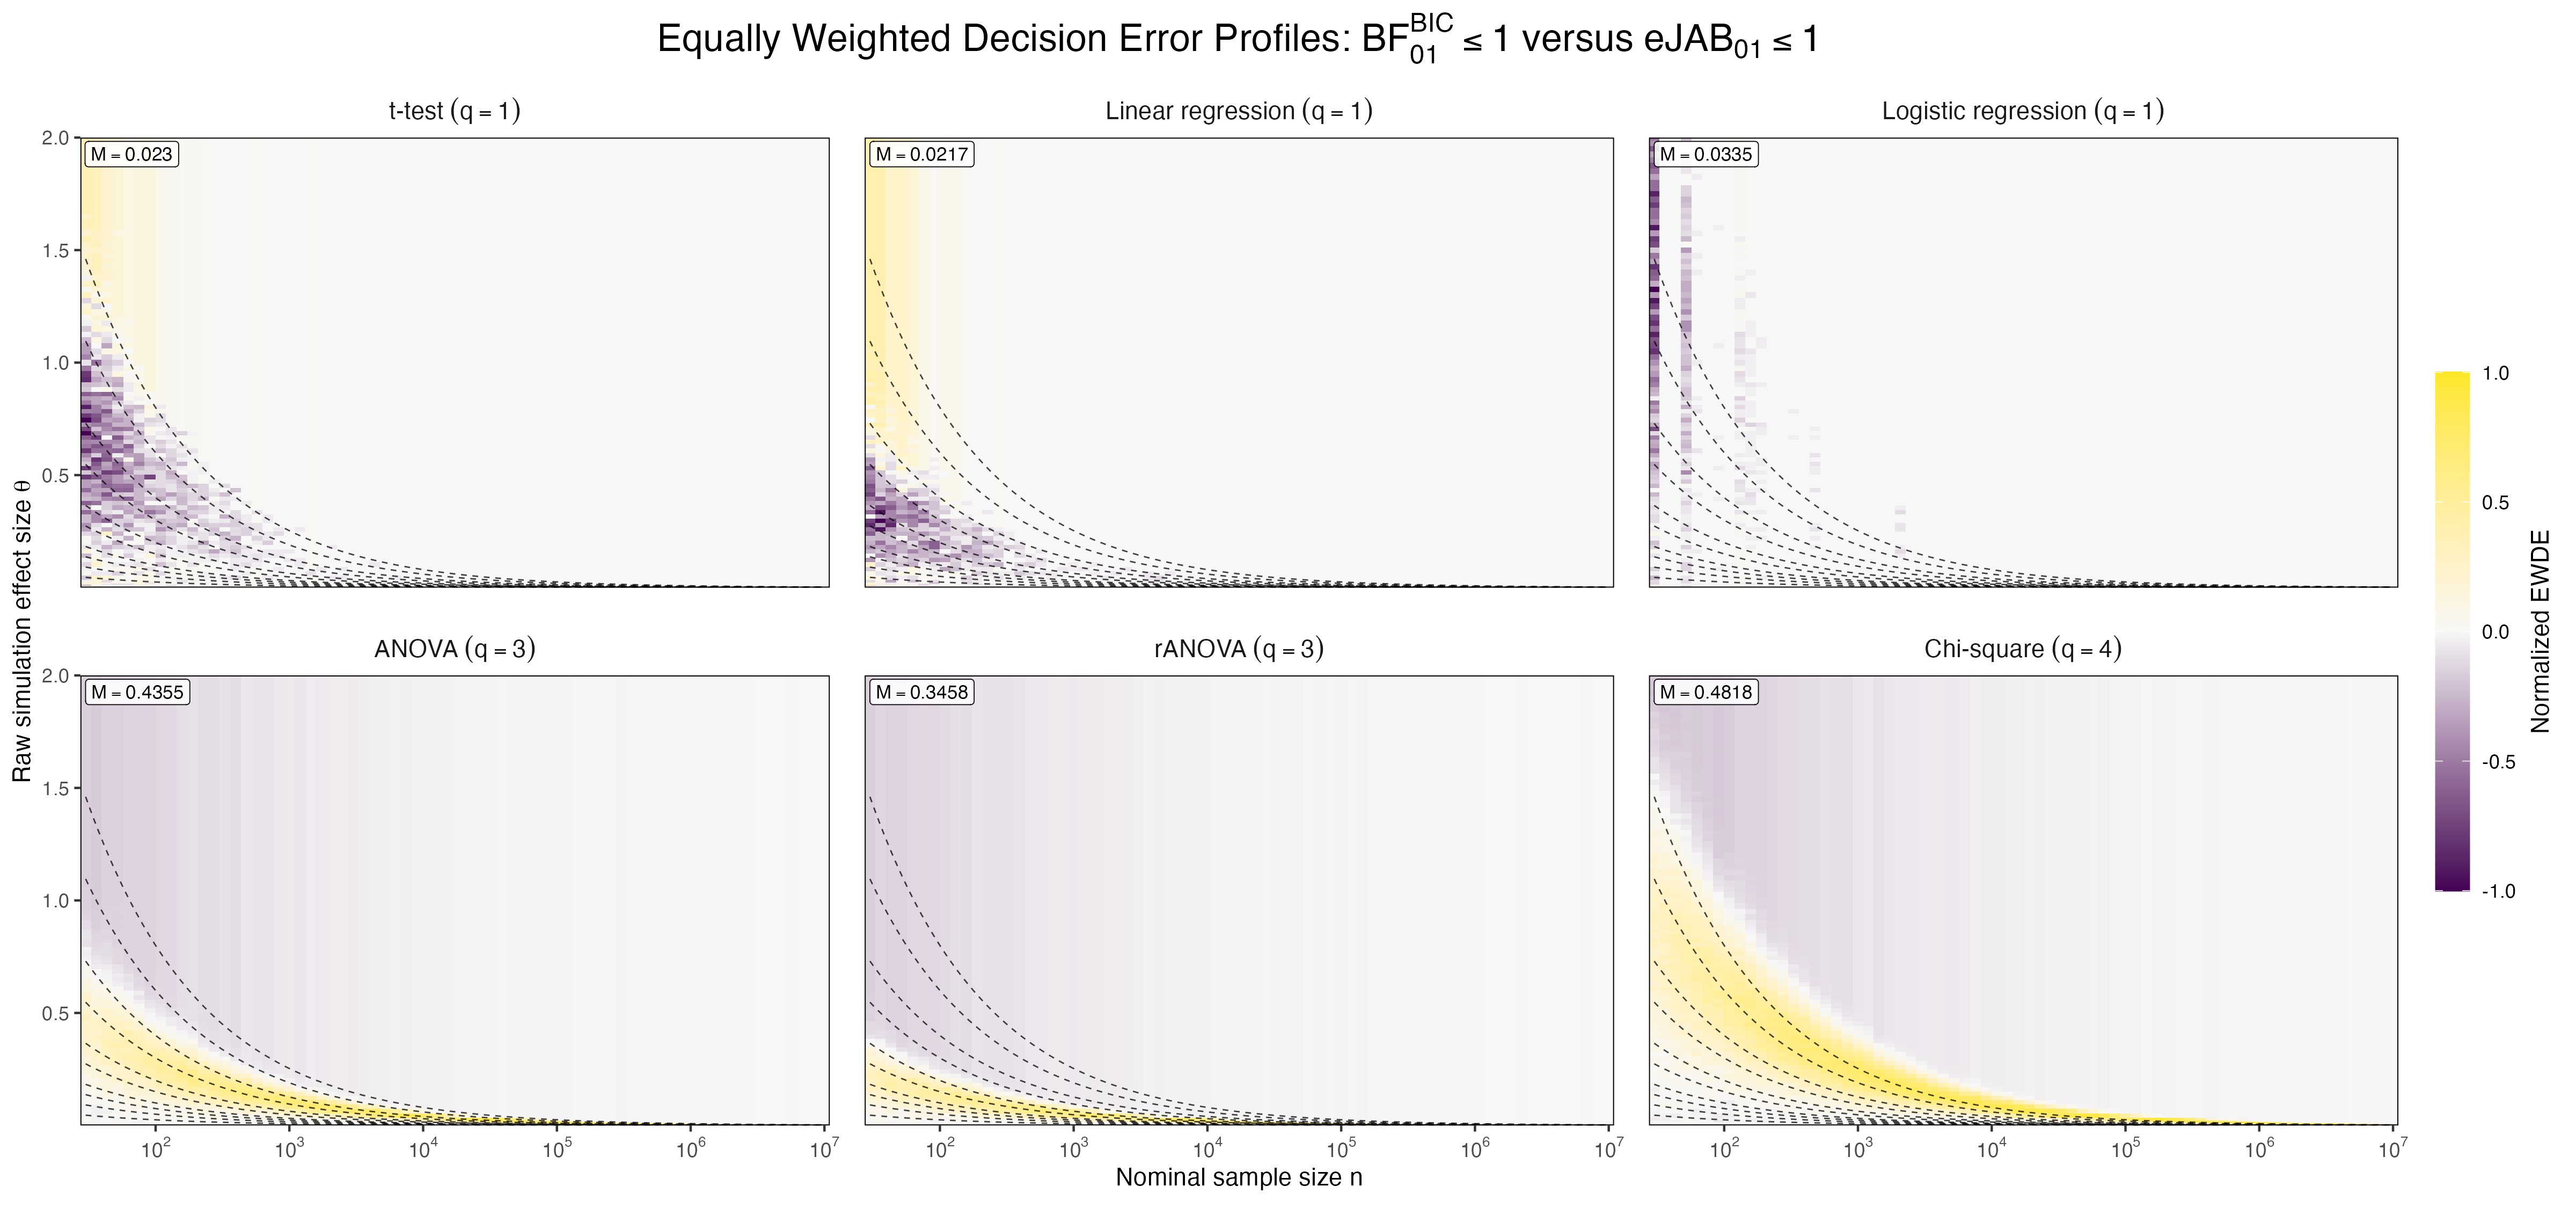
\includegraphics[width=\textwidth]{ewde_bic.png}
\caption{Equally Weighted Decision Error Profiles: additional comparisons.
Top: \(p<.005\) versus \(\ejab_{01}\leq1\) across ten tests.
Bottom: \(\BF_{01}^{\mathrm{BIC}}\leq1\) versus \(\ejab_{01}\leq1\)
for the six tests with an explicit parametric likelihood.
The BIC comparison excludes Cox regression and the three rank tests.
Colors show normalized EWDE. Positive values favor eJAB, and negative values favor the comparison
rule. The original panel-specific normalization constants are retained.}
\label{fig:additional-ewde}
\end{figure}
\clearpage
\bibliographystyle{plainnat}
\bibliography{references}
\end{document}
